\chapter{Project 1: NAND gate - bare metal approach} \label{ch:nand_bm}
Within this chapter I+it will be explained how to program a FPGA, in this specific case the one mounted on the KR260 starter kit, with the so-called bare metal approach.


\section{Vivado project}
Vivado is a software developed by AMD which is oriented to programming Field Programmable Logic Arrays - FPGAs - which supports various board and modules. It is a free software, even though an account is requested for the download(s).
\bigskip
\\The example project that will be discussed within this chapter is meant only to give an introduction to the Vivado-FPGA programming world, which is way more vast and deeper. The description is quite simple: a simple NAND gate which controls a user defined LED mounted on the development board.
\begin{figure}[ht]
	\centering
	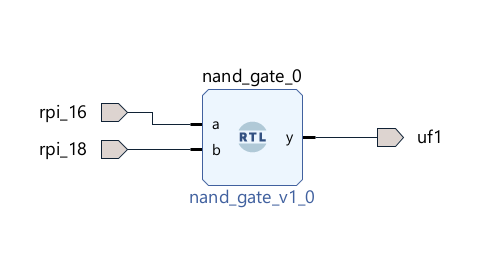
\includegraphics[width=0.65\textwidth]{images/prj1_1}
	\caption{NAND gate Vivado block design.}
	\label{fig:prj1_1}
\end{figure}
As it can be see the implementation is quite trivial, consisting only of one module, which is the behavioral description of the NAND gate.

\subsection{Project creation}
Once Vivado is open and the start page loaded, create a new project named \textbf{nand\_bm} (or whatever other name) and skip directly to the board selection window. In this window, select the name of the development board it is about to be used and create the project. The first two tasks to carry out are NAND gate behavioral description file creation and the physical constraint constraints definition.

\subsection{Behavioral description}
Move to \textbf{Sources} $\rightarrow$ \textbf{Design Sources} $\rightarrow$ right-click on this latter one $\rightarrow$ \textbf{Add Sources}. A window like the one shown in Figure \ref{fig:prj1_2} should appear.
\begin{figure}[ht]
	\centering
	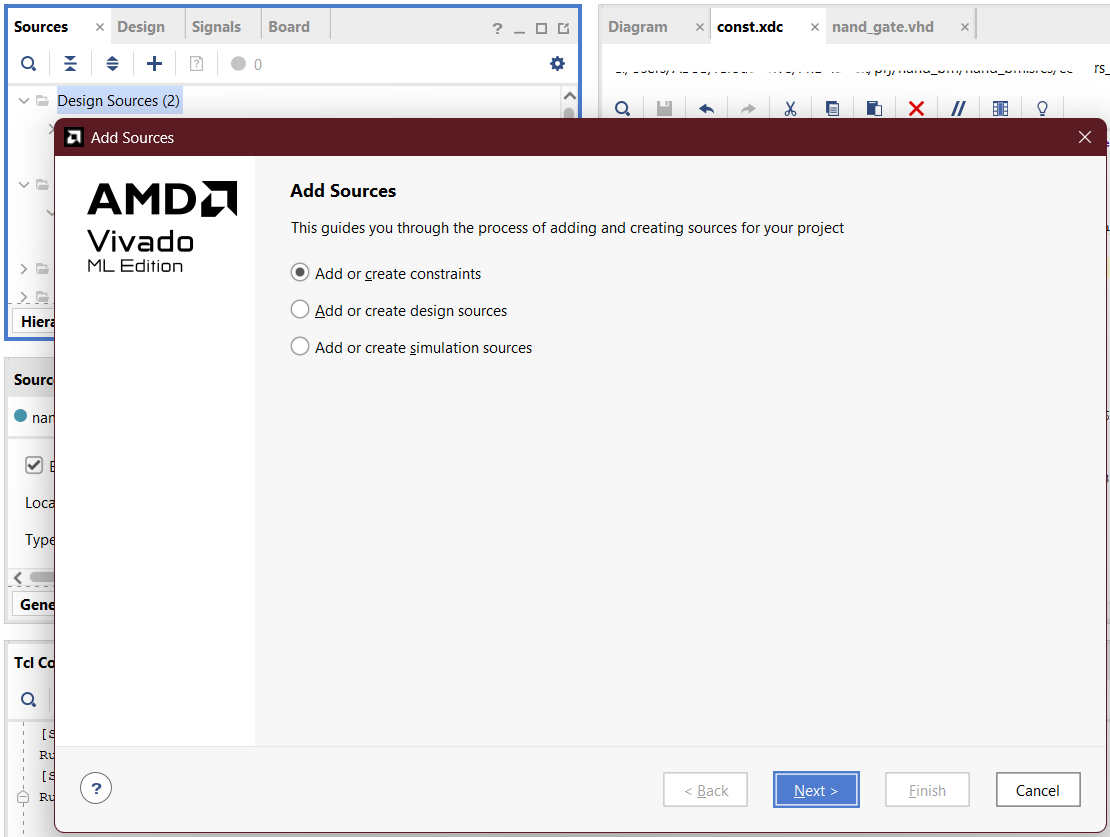
\includegraphics[width=\textwidth]{images/prj1_2}
	\caption{Add Sources window.}
	\label{fig:prj1_2}
\end{figure}
Select \textbf{Add or create design sources} $\rightarrow$ \textbf{Next} $\rightarrow$ \textbf{Create file} $\rightarrow$ enter the file name (nand\_gate) $\rightarrow$ \textbf{Finish}. Once it is done, a window to configure the inputs and the outputs of the gate should open. Such procedure can be skipped, providing that those information are defined in the description. The code to write down is the following:
\begin{verbatim}
	library IEEE;
	use IEEE.STD_LOGIC_1164.ALL;
	
	entity nand_gate is
	    Port ( a, b : in STD_LOGIC;
	              y : out STD_LOGIC);
	end nand_gate;
	
	architecture Behavioral of nand_gate is
	begin    
	    y <= a nand b;
	end Behavioral;
\end{verbatim} 
The project now has to be saved.

\subsection{Physical constraints}
The physical constraint file is the file that dictate which pin is connect to which within the development board and it of crucial importance for a real life application. Following a procedure similar to the one described for the behavioral description (\textbf{Sources} $\rightarrow$ \textbf{Constraints} $\rightarrow$ right-click on this latter one $\rightarrow$ \textbf{Add Sources} $\rightarrow$ \textbf{Add or create constraints} $\rightarrow$ \textbf{Next} $\rightarrow$ \textbf{Create file} $\rightarrow$ enter the file name (const) $\rightarrow$ \textbf{Finish}), the code to be written down is:
\begin{verbatim}
	set_property BITSTREAM.GENERAL.COMPRESS TRUE [current_design]
	
	#User defined pins
	set_property PACKAGE_PIN F8 [get_ports {uf1}]
	set_property IOSTANDARD LVCMOS18 [get_ports {uf1}]
	
	set_property PACKAGE_PIN AA12 [get_ports {rpi_16}]
	set_property IOSTANDARD LVCMOS33 [get_ports {rpi_16}]
	
	set_property PACKAGE_PIN Y9 [get_ports {rpi_18}]
	set_property IOSTANDARD LVCMOS33 [get_ports {rpi_18}]
\end{verbatim}
A bit of description it is needed to understand what those few lines of code do. The first line dictate that the bitstream that will be generated for this project will be compressed. The other lines define the port at which the buttons and the LED are connected (those information are provided from the datasheet of the board). For example, the pin at which the LED is connected is defined as a \textbf{standard I/O} with a voltage logic of \textbf{1.8V (LVCMOS18)}. In a similar way, the other two pins have the same characteristics, but with a voltage logic of \textbf{3.3V (LVCMOS33)}.

\subsection{Design generation}
Under the section of \textbf{IP INTEGRATOR}, click on \textbf{Create Block Design}: a new window will open. Move back to \textbf{Design Sources} $\rightarrow$ right click on the description file created earlier $\rightarrow$ \textbf{Add Module to Block Design}. To create a physical connection to the board pins, move the mouse tip on the block pins and type \textbf{Ctrl+T} to add a connection. By clicking on the created pins, a window named \textbf{External Port Properties} should appear. Rename those pins with the name define in the constraints file. Now the design should look like the one of Figure \ref{fig:prj1_1}

\subsection{FPGA programming}
To program the FPGA is needed a file that can be compared to the .hex file that will be generated for the programming of the a microcontroller (ATmega, STM32, ...). Move to the \textbf{PROGRAM AND DEBUG} section and click on \textbf{Generate Bitstream}. Follow the procedure and let the bitstream to be generated. The last step is to effectively program the device. Open the \textbf{Open Hardware Manager} and click on \textbf{Open Target} $\rightarrow$ \textbf{Auto Connect}, then click on \textbf{Program Device}.